\section{AVIST}
We implemented an animated visualization tool (AVIST) based on the GPU-centric design.
AVIST is written in C++, its computation codes are based on CUDA 7.5 and visualization codes are based on OpenGL and GLSL. The interface are coded by wxWidgets. We use the Thrust library\footnote{https://developer.nvidia.com/Thrust} for accelerating sorting, scaning, and reduction operations.

 

In this section, we give the implementation details of AVIST from four aspects: 1) the code organization of AVIST, which follows the Model-View-Controller (MVC) pattern and separates the system into three aspects: data transformations (model), data views and data filters (control); 2) data transformations, which feature the GPU parallel computing to achieve better performance; 3) correlated data views, which provide different visual aspects of multidimensional datasets; 4) user interactions, which emphasize  animation and cross-filtering for slicing big data into small.

\subsection{MVC Pattern}
The codes organization of AVIST follows the Model-View-Controller (MVC) design pattern as shown in Figure~\ref{fig:mvc}. The filters belong to the control part, which directly are applied to data views shown as the dash lines. The solid lines describe the method invocations. Firstly, filters trigger data models. Then, the data views are updated after the data model's change, thus they give users visual feedbacks.

\begin{figure}[htb]
	\centering
	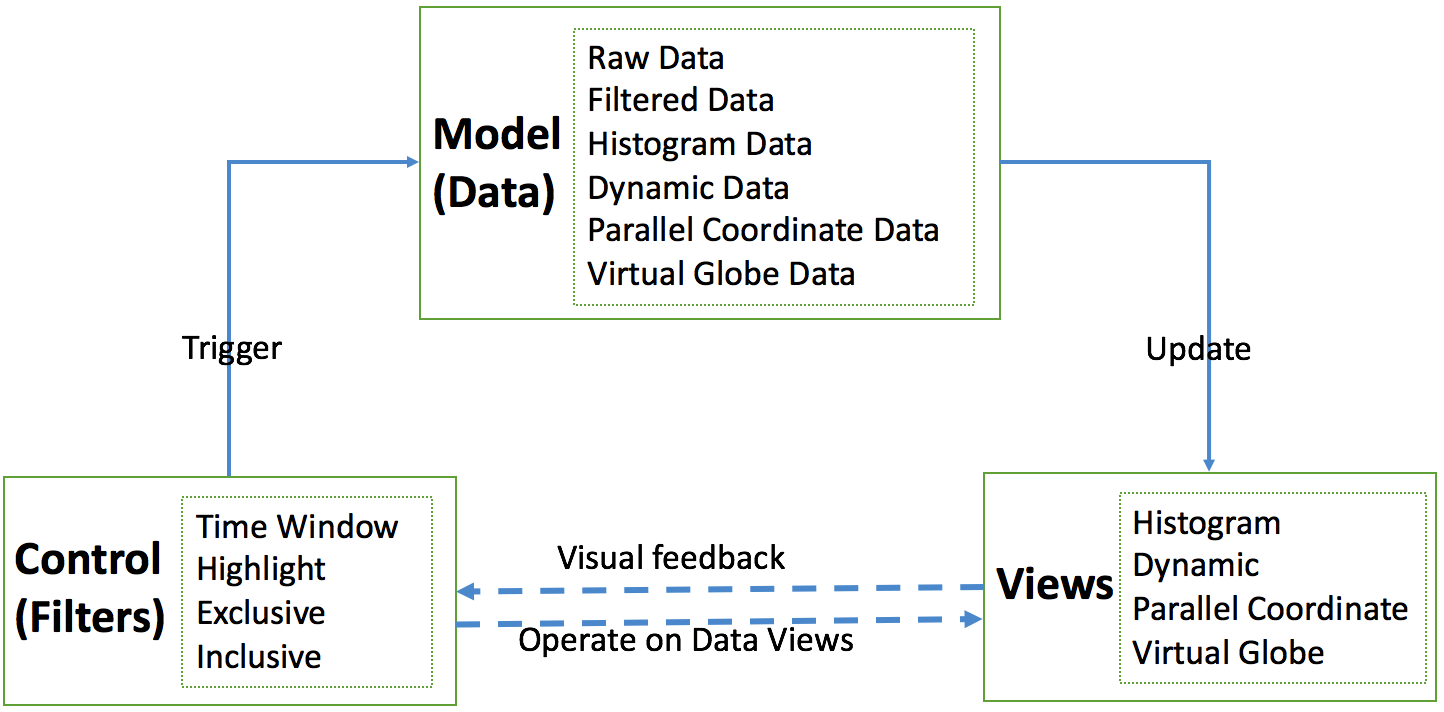
\includegraphics[width=1.0\linewidth]{pic/mvc.png}
	\parbox[t]{1.0\columnwidth}{\relax
	}
	%
	\caption{\label{fig:mvc} This figure shows the MVC design of AVIST. The dash lines show the visual operations and feedbacks between user interactions and data views. The solid lines describe the data path. First, filters trigger data model , then update the data views.  }
\end{figure}    


The MVC design pattern has several benefits. 1) We separate filters, data and views, which makes AVIST flexible to extend more filters, data transformations and data views in the future.  2) The model part is implemented on the GPU, which highlights the GPU-centric design. 3) The cross-filter design pattern can easily be  applied. User interactions of one data view can update the filters, which triggers the data transformations and updates other data views.


\subsection{Data Transformation}
AVIST features the GPU based vectorized data transformations. In this section, we describe data transformations following the data dependency graph design: data filtering, data processing and data rendering.

\subsubsection{Data filtering} 
This stage describes data transformations from raw data into filtered data as shown in Figure~\ref{fig:dataTran1}.
Firstly, a time window slices the raw data into a data snapshot, then data  filters are applied to the data snapshot to remove uninteresting records or highlight important ones. To boost performance, a binary search is applied for slicing data based on the data temporal locality.  The sliced data records are checked by data filters in parallel, and then they are reduced to the filtered records.   

\begin{figure}[htb]
	\centering
	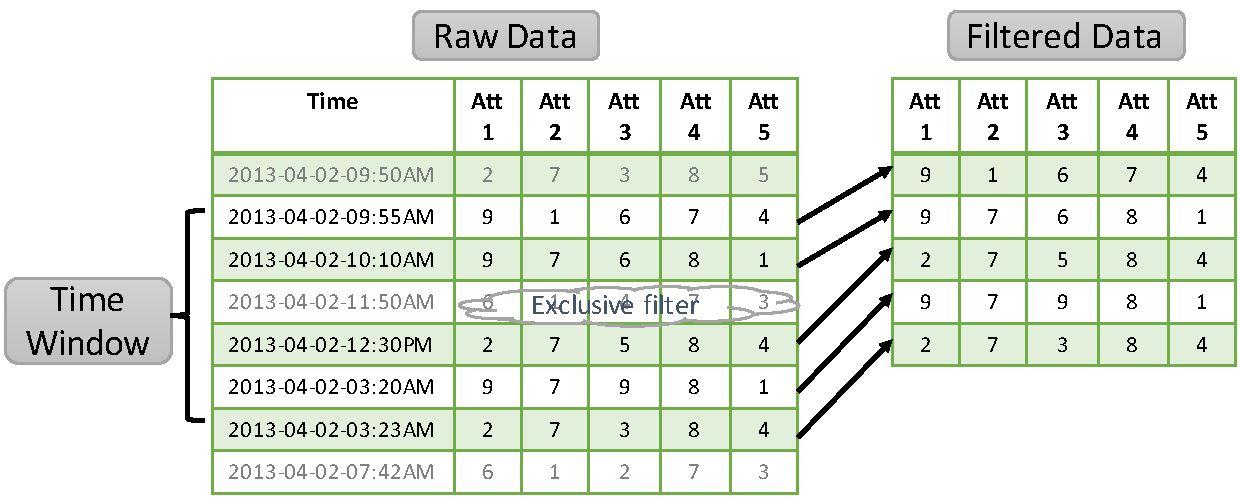
\includegraphics[width=1.0\linewidth]{pic/trans.pdf}
	\parbox[t]{1.0\columnwidth}{\relax
	}
	%
	\caption{\label{fig:dataTran1} Data transformations from raw data to filtered dataset.}
\end{figure} 




\subsubsection{Data processing}
The computations of data processing and rendering are view dependent. We demonstrate the detailed implementation of four data views: histogram view, time-series view, parallel coordinate plots and virtual global view (the descriptions of them are provided in section 4.3).

\begin{figure}[htb]
	\centering
	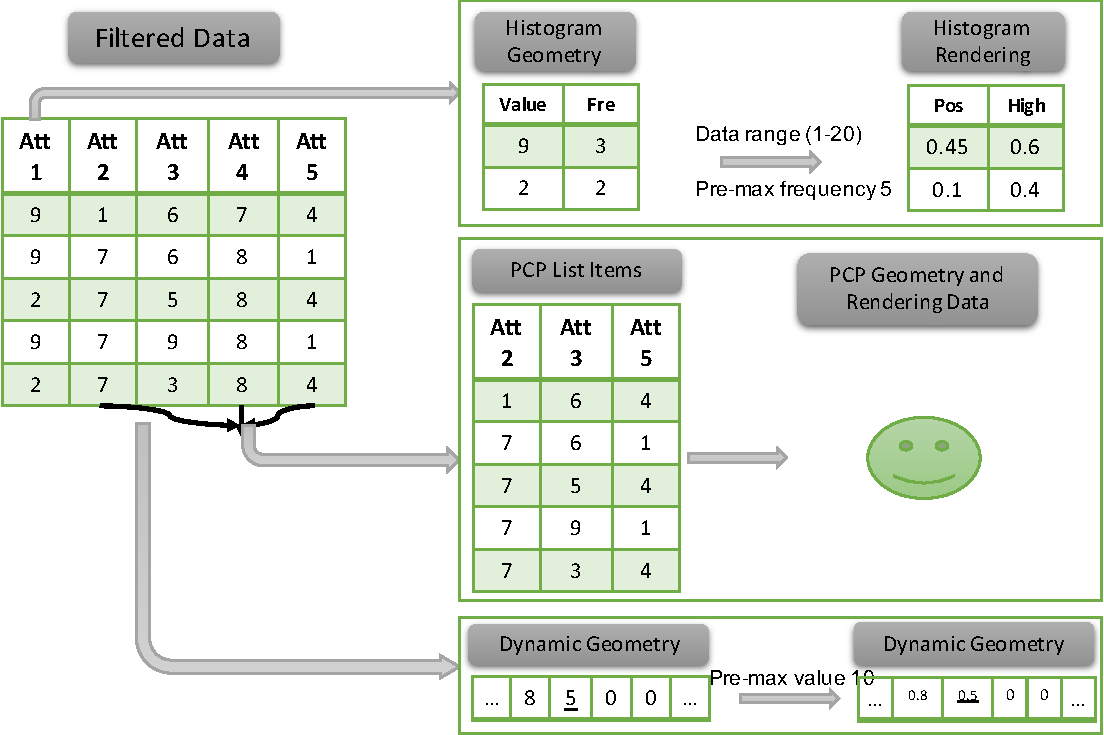
\includegraphics[width=1.0\linewidth]{pic/tran2.pdf}
	\parbox[t]{1.0\columnwidth}{\relax
	}
	%
	\caption{\label{fig:dataTran2} Data transformations from filtered data into visual primitives.}
\end{figure} 


\begin{figure}[htb]
	\centering
	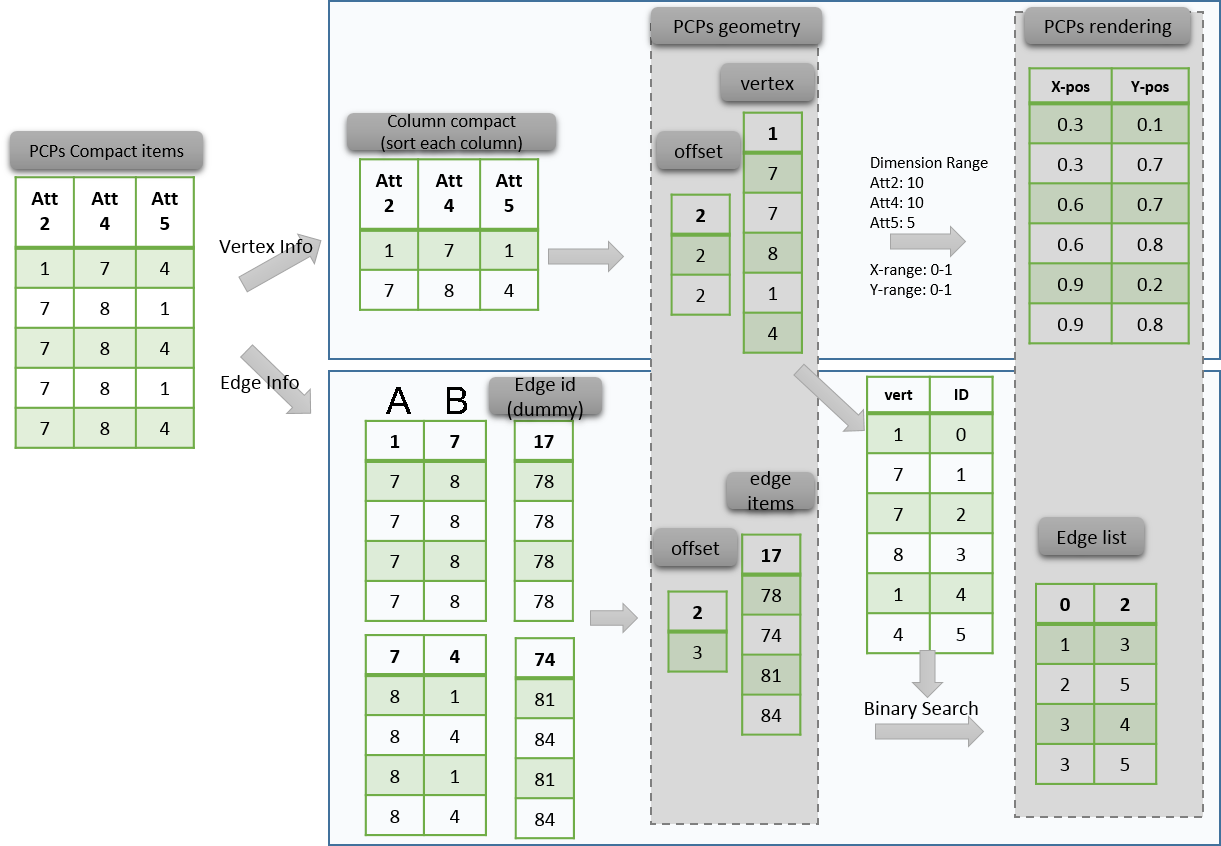
\includegraphics[width=1.0\linewidth]{pic/trans3.pdf}
	\parbox[t]{1.0\columnwidth}{\relax
	}
	%
	\caption{\label{fig:dataTran3} This figure shows data transformations from compact item lists to rendering data in parallel coordinate views. The data transformations are separated into two parts: vertex and edge.}
\end{figure} 

Figure~\ref{fig:dataTran2} demonstrates data transformation of histogram and dynamic views. Based on the users' chosen column, AVIST retrieves this column data,  aggregates them, and visualizes them. The steps are described as follows. 
\begin{enumerate}[noitemsep]
	\item Sort the  column to obtain unique values and their frequency.
	\item Get X position of each unique value based on the data range.
	\item Get Y position of each unique value based on previous maximum frequency.
\end{enumerate}	

Data transformations of  time-series view is straightforward: the GPU counts the number of  filtered data items, then transforms it to height value (based on previous maximum value). 

Data transformations of parallel coordinate plots (PCPs) are more complex than other views. After the GPU generates PCPs compact items based on chosen axes, the data flow is separated into two parts as shown in Figure~\ref{fig:dataTran3}. The steps for generating vertex of PCPs:
\begin{enumerate}[noitemsep]
	\item  Sort  columns to obtain unique values.
	\item Compact  columns' unique values into \textit{vertex} array with their size \textit{offset} array.
	\item Generate Y-axis positions based on the data dimensions' range, and X-axis positions based on the axis chosen order. 
\end{enumerate}

The steps for generating edge list of PCPs are as follows:
\begin{enumerate}[noitemsep]
	\item Two neighboring columns are grouped into one array, which is \textit{Edge ID} list. The values of list are called dummy values and calculated by: 
	
	$dummyValue = value_{columnA}*range_{columnA} + value_{columnB}$
	
	\item  Sort \textit{Edge ID} lists to obtain unique values.
	\item Compact each list's unique values into \textit{edge} array with their size \textit{offset} array.
	\item Split \textit{edge} array into two arrays with vertex values of their columns.
	\item Replace vertex values with their orders based on \textit{vertex} array.
	
\end{enumerate}

The virtual global view is a special case of parallel coordinate views with two axes. The difference is that vertex position is 3D in virtual global view. And there are extra steps for generating 3D positions based on longitudes and latitudes. 
The lines are Bezier curves, which are generated based on virtual globe size and the strategies of selecting control points.


\subsubsection{Data rendering}
After generating visual primitives, AVIST maps them into the GPU vertex buffer objects. The  GPU VBOs offer substantial performance gains and avoid data transformations between main memory and GPU memory.

However,  visual primitives in VBOs are vertexes and edges. In order to  generate rectangles, areas or more advanced shapes, we use GLSL for post-processing. For example, we split one vertex into four vertexes to generate rectangles in histogram view. We also transform vertexes into line strip to generate areas in time-series view.


\subsection{Correlated Data Views}
Four data views are implemented in AVIST, which can provide different visual aspects of the multidimensional datasets.

\begin{itemize}
	
	
	\item \textbf{Histogram view} shows  data distribution of  sliced data snapshot. Analysts can select different dimensions  from a listbox to explore different aggregation information.
	
	\item \textbf{Time-series view} shows the data aggregation of certain filtered events over a period of time. When an analyst change his or her data filters, the time-series view clears previous results and re-draw everything. 
	
	\item \textbf{Parallel coordinate plots} show  details of each data record. Analysts can select multiple data dimensions to generate their custom parallel coordinate plots. The axes are organized based on their selected order in the listbox.
	
	\item \textbf{Virtual global view} shows the data geography distributions.  A Bezier curve links two locations on the virtual global for showing their  relationships.
	
\end{itemize}

The data views works together with data filters, to be enable cross-filtering of multidimensional datasets, which makes those data views correlated. Those data views support directly visual filtering with brushing interactions (e.g., an analyst firstly select highlight filter with solo mode,  then he brush one bar in histogram view to highlight related data records).


\subsection{User Interactions}
AVIST is an exploration oriented visual analysis tool, which highlights animation and cross-filtering for exploring time-series and multi-dimensional datasets. Figure~\ref{fig:control} is the control panel of AVIST,  which shows the detailed user interactions. 

\begin{figure}[htb]
	\centering
	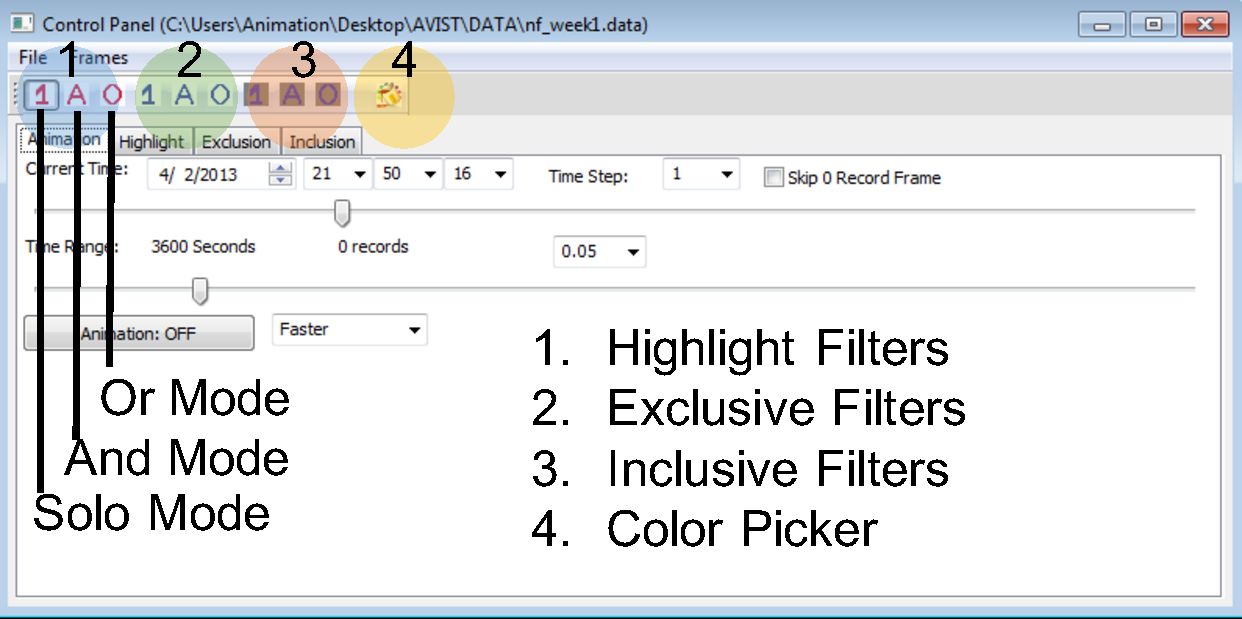
\includegraphics[width=1.0\linewidth]{pic/control.pdf}
	\parbox[t]{1.0\columnwidth}{\relax
	}
	%
	\caption{\label{fig:control} The control panel of AVIST. Three filters (\textit{highlight filter, exclusive filter} and \textit{inclusive filter}) with three modes (\textit{solo} mode, \textit{and} mode, and \textit{or} mode) are provided. }
\end{figure} 

%\begin{itemize}
	\subsubsection{Animation}
	The animation interactions include automatic forward playback, interactively dragging of the time window bar, and interactive change of animation speed. By changing the current time and time range, the time window is customized  to slice data into snapshots, which will be analyzed and visualized at the correlated data views. By combining automated animation with these correlated views, AVIST can provide temporal changes in the datasets, which supports  discovery temporal patterns for further analysis.
	\subsubsection{Filtering}
	Three different filters are implemented in AVIST (their usabilities are shown in following case studies).
	\begin{enumerate}[noitemsep]
		\item \emph{highlight filters}, which make the selected data items stand out of the rest data with different colors.
		\item \emph{exclusive filters}, which remove uninteresting data  items.
		\item \emph{inclusive filters}, the exact opposite of exclusive filters, which remove all data items except those marked by an analyst.
	\end{enumerate}
	Each data filter has three modes: 
	\begin{enumerate}[noitemsep]
		 \item \emph{solo} mode , which allows only one filter item in current filter set.
		 \item \emph{and} mode, which combines several filters together as a whole for emphasizing that data records need satisfy all requirements.
		 \item \emph{or} mode, which means that data records just need to meet only one of the filter requirements.
	\end{enumerate}
	 Based on these three basic filters with their three modes, analysts can nest them to generate complex data filters and apply them to different data views,  which help them to drill down each piece of data record to ``find a needle"  on demand. %These filtering interactions are implemented for each data view to support cross filtering, which enables analysts to reveal hidden insights.


	\subsubsection{Capacities}
The animation interactions can slice  high velocity data into fine-grained subsets by narrowing down the size of time windows; filtering interactions can extract relevant records for concentrating small subsets of high volume data. These interactions transform the large data into small size by removing uninteresting items or highlight important ones, which ensures the flexibility of exploring large multidimensional datasets. In all, AVIST highlights animation and cross-filtering for exploring data by considering its big volume and high velocity features.







